
\documentclass[11pt]{article}

\usepackage{common}
\usepackage{amsfonts}
\usepackage{hyperref}
\title{HW3: Language Modeling}
\author{Colton Gyulay \\ cgyulay@college.harvard.edu }
\begin{document}

\maketitle{}
\section{Introduction}

In the third problem set, our goal was to implement various language models in order to predict words given previous contexts. At a high level, this task seeks to develop models that narrow down possible following words in order to build more succinct representations for language as a whole. This context built of preceding words was the only input we used for our models, which can be cleanly divided into two primary methodologies: n-gram language models and neural language models. The n-gram language models are built with Markovian assumptions, while the neural models follow the work of \citet{DBLP:journals/jmlr/BengioDVJ03}.

The first class of models were comprised of simple n-gram count-based approaches (CBLMs), with relatively small context sizes. These were improved upon through Laplacian and Witten-Bell interpolative smoothing. The second class of models were utilized neural network approaches (NNLMs), and notably attempted to learn dense embeddings for each word in order to improve on the prediction task.

The CBLMs were able to achieve fairly low perplexity with incredibly little training time (a single pass over the data to build a count matrix). They were, however, confounded far more often than NNLMs by contexts and words previously unseen in training. This resulted in a large divergence between training and validation perplexity for the count-based models, a phenomenon that was not as pronounced in the neural models.

\section{Problem \& Model Descriptions}

\subsection{Dataset}

The primary training dataset used was the Penn Treebank, which contained around $900,000$ words. This dataset was simplified by limiting total vocabulary $\mcV$ to 1,000 words in one training set (PTB1000), and to 10,000 words in another (PTB). All words were treated as lower case only, while padding on either end of examples was mapped to special start and stop tokens, allowing models to predict first and final words. All words appearing outside the limited vocabulary were mapped to a single "unknown" token. Artificially limiting the vocabulary allows for inflated results in regard to perplexity over the dataset, but this sacrifice was necessary in the face of lengthy training time requirements. Sentences in the dataset were divided into context subsets of size $d_{win}$ = 2, 3, and 6, where the assigned label was the final word in the context.

\subsection{N-gram Language Models}

We built multiple variations of n-gram language models, each of which differed in their handling of unseen contexts/words. Unigram, bigram, and trigram context/word co-occurrence matrices were built: $\boldF_{uni} \in \reals^{|V|}$, $\boldF_{bi} \in \reals^{|V| x |V|}$, and $\boldF_{tri} \in \reals^{2|V| x |V|}$. The first model (MLEUniform) used maximum likelihood estimation by examining contexts and predicting the highest probability following words based on occurrences in the training corpus. When a context appeared in test that was previously unseen in training, probability defaulted to a uniform distribution of words from $|\mcV|$.

A second model (MLEUnigram) closely followed which defaulted to the unigram distribution in the case of unseen contexts. For seen contexts but unseen words, these probabilities were normalized for each context. The third model (CBLap) used a Laplacian smoothing constant $\alpha$ to provide non-zero probabilities to unseen context/word occurrences.

Our third model interpolated between multiple levels of context distributions, combining information from trigram, bigram, and uniform distribution to pick the most likely word (CBWB). The balance of interpolation was informed by Witten-Bell smoothing. At a high level, a word probability can be formalized as follows:
\begin{center}
    $p(w_{\scriptscriptstyle i}|w_{\scriptscriptstyle i-n+1},...,w_{\scriptscriptstyle i-1}) = \boldF[w_{\scriptscriptstyle i-n+1},...,w_{\scriptscriptstyle i-1}]$
\end{center}

The balance between distributions outlined by Witten-Bell smoothing can be formalized like so (where $c = w_{\scriptscriptstyle i-n+1},...,w_{\scriptscriptstyle i-1}$). Each $\lambda_{i}$ is determined based on prevalance of that context and word pair at each different context length, and are normalized to sum to 1 to ensure convex combination:
\begin{center}
$p(w_{\scriptscriptstyle i}|c) = \lambda_{1}\boldF_{tri}[c] + \lambda_{2}\boldF_{bi}[c'] + \lambda_{3}\boldF_{uni}[c'']$
\end{center}

\subsection{Neural Language Models}

Moving on from the more naive count-based approach, we built neural language models leveraging the topology outlined by \citet{DBLP:journals/jmlr/BengioDVJ03}. Count-based models become difficult to manage as $d_{win}$ increases due to overwhelming the sparsity of $\boldF$. NNLMs overcome this problem by learning parameters to model the underlying distribution, rather than by performing strict counts. This allowed us to increase our input to $d_{win} = 6$, essentially a preceding context of 5 words, without memory issues. To generate a predicted distribution, the context words were first fed into a lookup table which held learned word embeddings $\boldW^{0} \in \reals^{|V| x |e_{i}|}$ (embeddings $e_{i} \in \reals^{30}$). These results were concatenated into input $\boldx \in \reals^{d_{win} x |e_{i}|} (\reals^{d_{in}})$. At this point $\boldx$ was fed through a linear layer with weights $\boldW^{1} \in \reals^{d_{in} x d_{hid}}$ and $\boldb^{1} \in \reals^{d_{hid}}$, a tanh layer, and a final linear layer with weights $\boldW^{2} \in \reals^{d_{hid} x |V|}$ and $\boldb^{2} \in \reals^{d_{|V|}}$. Predictions were then normalized using \textit{logsoftmax}, which normalizes by dividing each entry by the sum  of log probability prediction. The model can be formalized as follows:
\begin{center}
    $NNLM(x) = logsoftmax(tanh(\boldx\boldW^{1} + \boldb^{1})\boldW^{2} + \boldb^{2})$
\end{center}

As \textit{logsoftmax} requires summing over the total $\mcV$ for each example, training can be quite slow. We experimented with \textit{hierarchical logsoftmax}, which is defined cleanly in \citet{DBLP:journals/corr/MikolovSCCD13}. Essentially, we sorted the vocabulary into a 2-layer tree, assigning each word first to a branch. We chose a random, 2-layer tree with approximately $\sqrt{|V|}$ branches and $\sqrt{|V|}$ leaves per branch. This slightly different model topology (NNLMHSM) is visualized further in the next section.

\section{Model Structure \& Training}

A high level description of each model was given in the previous descrption, and here we will more formally present the topology and code used to build each of our models. The count-based language models primarily utilized context/word co-occurrence matrices, for which the Torch code is as follows:
\begin{verbatim}
function build_ngram(x, y)
  -- Building p(w_i|w_i-n+1,...,w_i-1)...
  local ngram = {}
  for i = 1, x:size(1) do
    local ctx = tensor_to_key(x[i])
    local wi = y[i]
    local val = ngram[ctx]
    if val == nil then
      ngram[ctx] = {}
      ngram[ctx][wi] = 1
    else
      local innerval = ngram[ctx][wi]
      if innerval == nil then
        ngram[ctx][wi] = 1
      else
        ngram[ctx][wi] = ngram[ctx][wi] + 1
      end
    end
  end
  return ngram
end
\end{verbatim}

The Torch implementation of the basic NNLM closely follows the mathematical formalization above. The model below used our primary embedding and weight sizes, of size $e=30$ and $d_{hid} = 100$, respectively. The final linear layer shows a mapping to the limited vocabulary of PTB1000 ($|\mcV| = 1000$).
\begin{verbatim}
nn.Sequential {
  [input -> (1) -> (2) -> (3) -> (4) -> (5) -> (6) -> output]
  (1): nn.LookupTable
  (2): nn.View(150)
  (3): nn.Linear(150 -> 100)
  (4): nn.Tanh
  (5): nn.Linear(100 -> 1002)
  (6): nn.LogSoftMax
}
\end{verbatim}

The Torch implementation of the hierarchical softmax NNLM followed the topology of the previous model closely, with the one exception that the output was log probability only for a specific leaf. Information regarding leaf lookup was passed directly to the final layer through the use of a parallel table:
\begin{verbatim}
nn.Sequential {
  [input -> (1) -> (2) -> output]
  (1): nn.ParallelTable {
    input
      |`-> (1): nn.Sequential {
      |      [input -> (1) -> (2) -> (3) -> (4) -> (5) -> output]
      |      (1): nn.LookupTable
      |      (2): nn.Reshape(150)
      |      (3): nn.Linear(150 -> 100)
      |      (4): nn.Tanh
      |      (5): nn.Linear(100 -> 1002)
      |    }
      |`-> (2): nn.Identity
       ... -> output
  }
  (2): nn.SoftMaxTree
}
\end{verbatim}

\subsection{Training}
As mentioned, count-based models required only a single epoch of training to learn context/word probability associations. NNLM training took significantly more time and resources, and primarily utilized mini-batch stochastic gradient descent with a batch size of 32. Training was done using the Torch library optim, which was able to achieve reasonable epoch times (~6 minutes) even when summing over $\mcV$ for the full PTB dataset.

\subsection{GPU Training}
We would be remiss not to mention how much time was spent prepping our models for GPU compatible training. Unfortunately, the end result was naught. We struggled to track down memory errors, and even with a further study into garbage collection could not overcome cuda runtime errors relating to memory. The model's structure may not have been 100\% correct, but there didn't seem to be Lua memory errors \textemdash  only cuda ones. We hope to have this resolved for the next assignment in order to boost training speed even further. As it stood, CPU training was not necessarily prohibitive.

\subsection{Evaluation}
For this specific task of language modeling, each model was evaluated on the metric of perplexity. Intuitively, perplexity can be thought of as how confident/confused a model is about its predictions given a specific context. Mathematically, this is represented by the exponential of the average negative log-likelihood over $n$ context/word examples:
\begin{center}
    $perp = exp(-\frac{1}{n}\sum_{i=1}^{n} p(w_{\scriptscriptstyle i}|w_{\scriptscriptstyle i-n+1},...,w_{\scriptscriptstyle i-1}))$
\end{center}

\section{Experiments}

Interestingly, our Witten-Bell smoothing CBLM model performed the best. The count-based models were far less generalized than the NNLM models and saw a large divergence between training and validation accuracy. This is largely attributable to how these models handle unseen contexts/words. Our NNLMs generalized well and approached the performance of the best count-based model, but were unable to surpass it. Overall, our best model on the full PTB dataset achieved a validation perplexity of 234.01 using Witten-Bell smoothed bigrams/unigrams. The basic NNLM achieved similar performance on the limited vocabulary dataset, which implies that with longer training/further optimization we might be able to generate comparable scores on the full PTB.

\subsection{CBLMs}
The only hyperparameter we tuned for a CBLM was the $\alpha$ Laplacian smoothing constant used in our CBLap model. We found that a relatively small amount of smoothing was optimal \textemdash  the best-performing model used $\alpha = 0.01$. As long as all contexts had been seen, as on the training dataset, for example, continuously decreasing the smoothing constant resulted in lowered perplexity. On validation, however, a more generalizable medium was found.

\begin{center}
    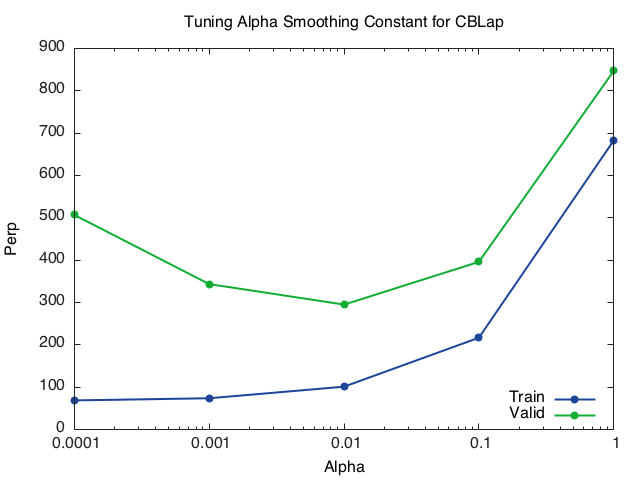
\includegraphics[width=12cm, length=10cm]{laptune.png}\\
    \textit{Figure 1: Tuning hyperparameter $\alpha$ for CBLap 2-gram.}
\end{center}

The complete results of our n-gram count-based models on PTB and PTB1000 can be seen in \textit{Table 1}. The best performing model on the full vocabulary validation dataset was the Witten-Bell smoothed bigram.

\begin{table}[h]
\centering
\begin{tabular*}{0.75\textwidth}{@{\extracolsep{\fill} }| c | c | c | c | c |}
 \toprule
 Model & PTB1k (T) & PTB1k (V) & PTB (T) & PTB (V)\\
 \midrule
 \textsc{MLEUniform2} & 33.65 & 49.21 & 68.67 & 511.19\\
 \textsc{MLEUniform3} & \textbf{14.73} & 71.51 & \textbf{9.79} & 1548.37\\
 \textsc{MLEUnigram2} & 33.65 & 49.21 & 68.67 & 506.66\\
 \textsc{MLEUnigram3} & \textbf{14.73} & 65.19 & \textbf{9.79} & 885.10\\
 \textsc{CBLap2} & 33.95 & 44.96 & 216.82 & 294.94\\
 \textsc{CBLap3} & 18.81 & 52.84 & 71.02 & 605.19\\
 \textsc{CBWB2} & 38.85 & \textbf{44.67} & 122.63 & \textbf{234.01}\\
 \textsc{CBWB3} & 30.58 & 61.04 & 34.02 & 337.27\\
 \bottomrule
\end{tabular*}
\caption{\label{tab:results} Validation perplexity results from all models. Suffix numbers refer to n-gram length.}
\end{table}

\subsection{NNLMs}

In regard to NNLMs, we experimented primarily on three fronts: learning rate $\eta$, embedding size $e$, and output activation (\textit{logsoftmax} vs. \textit{hierarchical logsoftmax}). Consistent with our findings last week, we found the optimal $\eta$ to be 0.01. \citet{DBLP:journals/jmlr/BengioDVJ03} used an embedding size of 30, though we were able to improve our results with an embedding size increased to 50. Our best performing NNLM was trained with $e=50$, $\eta=0.01$, and mini-batches of size 32 over 15 epochs. This specific model recorded a validation perplexity of 297.16.

\begin{center}
    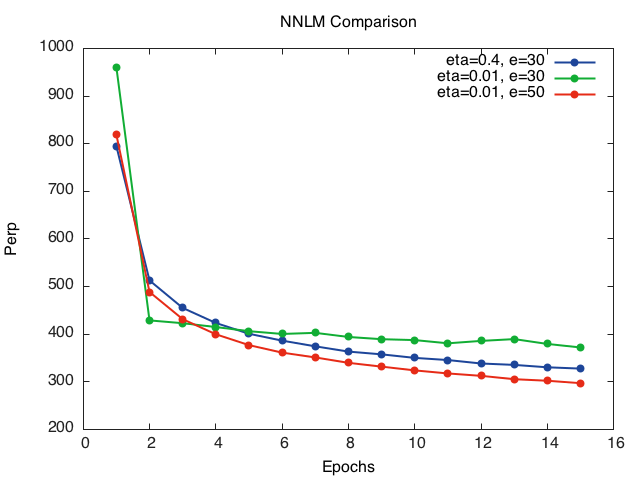
\includegraphics[width=12cm]{nnlmcomp.png}\\
    \textit{Figure 2: Comparing NNLM hyperparameters.}
\end{center}

Unfortunately, we were unable to push the results of NNLMs beyond count-based approaches due to inaccuracies with the implementations of noise-contrastive estimation and \textit{hierarchical logsoftmax}. Though we were able to get the NNLMHSM model working on the limited vocabulary dataset, we could not replicate this training with the larger dataset. Given the promising performance on PTB1000, given more time and tuning these models would have surpassed count-based approaches. A comparison of the two NNLM variants can be seen in \textit{Figure 3} as well as in \textit{Table 2}.

\begin{center}
    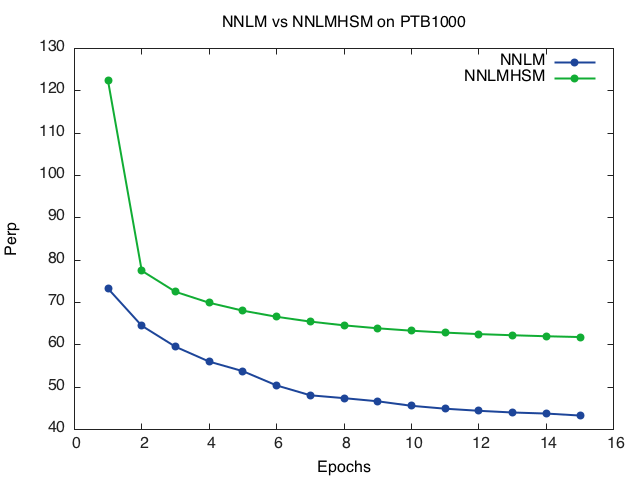
\includegraphics[width=12cm]{nnlmcomp1000.png}\\
    \textit{Figure 3: NNLM vs NNLMHSM on PTB1000.}
\end{center}

\begin{table}[h]
\centering
\begin{tabular*}{0.5\textwidth}{@{\extracolsep{\fill} }| c | c | c |}
 \toprule
 Model & PTB1k & PTB\\
 \midrule
 \textsc{NNLM6} & \textbf{43.28} & \textbf{297.16}\\
 \textsc{NNLMHSM6} & 67.42 & --\\
 \bottomrule
\end{tabular*}
\caption{\label{tab:results} Validation perplexity results from NNLMs. Suffix numbers refer to n-gram length.}
\end{table}

\subsection{Embeddings}

The input embedding matrix $\boldW^{0}$ is of particular interest as its weights are essentially learned vector representations for words. After teach training epoch, we enforced a max $l_{2}$ norm of 1 on each embedding, ensuring relatively equivalent magnitudes. We experimented with two different vector similarity techniques \textemdash  dot product and cosine similarity. Using k-nearest neighbors we are able to extract which words the model "believes" to be similar. Even with the $l_{2}$ norm threshold, we found that accounting for magnitude lowered the quality of these comparisons, so we opted for cosine similarity, which only accounts for directional equivalence. A few examples of nearest neighbors are as follows (word, similarity score):

\begin{itemize}
  \item company: government (0.883), japan (0.880), carrier (0.870), fed (0.864), concern (0.860), agency (0.852), country (0.837)
  \item know: think (0.951), say (0.944), clear (0.924), saying (0.922), wonder (0.918), surprised (0.911), though (0.908)
  \item june: april (0.992), march (0.983), july (0.981), november (0.979), october (0.971), december (0.966), february (0.965)
  \item germany: britain (0.979), japan (0.945), mexico (0.945), quebecor (0.942), ibm (0.935), gm (0.935), france (0.934)
  \item unhappy: 1930s (0.921), wars (0.916), adjustments (0.914), identified (0.912), alive (0.910), nerves (0.910), land (0.909)
\end{itemize}

Though these embeddings are not as high quality as those produced by \citet{DBLP:journals/corr/MikolovSCCD13}, they still indicate that the model is learning successfully. Comically, it tends to blur the lines between countries and companies, perhaps not so differently than the close political and commercial relationships we see in today's world.

\section{Conclusion}

In conclusion, we were able to achieve okay results with our neural approach. Nevertheless, our NNLM was able to produce decent embeddings which would be serviceable for use upstream in other applications. As in the last pset, we found the topology and hyperparameters outlined by \citet{DBLP:journals/jmlr/BengioDVJ03} to be quite good already, though we were able to find improvements by increasing embedding size. Regrettably we did not have great success with the techniques noise-contrastive estimation nor hierarchical softmax.

We were able to generate stronger results with count-based language models, especially using Witten-Bell smoothing with interpolation between multiple n-gram contexts. This assignment demonstrated the importance of the training data in supervised learning, as count-based models performed much better when all contexts/words had been previously encountered. The NNLM approach allowed for better generalization than these models could offer, even with more advanced smoothing approaches.

This assignment posed a particular difficulty to my team (me), and I was a little disappointed at the final results in relation to the time put in. Many aspects of the NNLM I felt were close to being there (i.e., hierarchical softmax, GPU training), though not perfected. All code can be found on GitHub here \url{https://github.com/cgyulay/cs287/tree/master/HW3}, while Kaggle submissions can be found under the team name "Potato Farmers".

\bibliographystyle{apalike}
\bibliography{writeup}

\end{document}
